\begin{figure}[h]
   \centering
   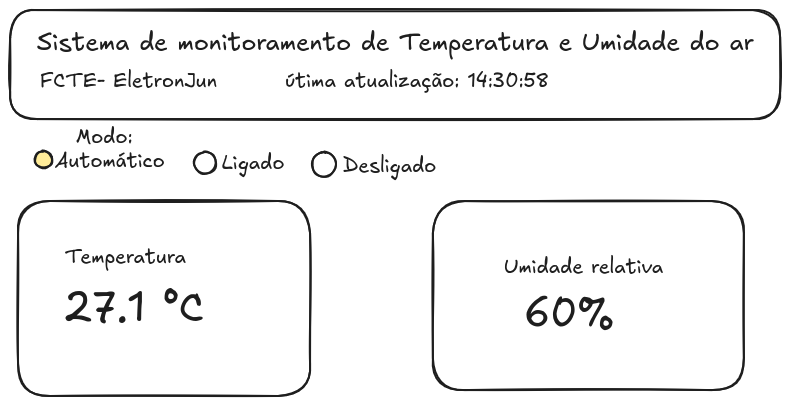
\includegraphics[width=0.8\textwidth]{imagens/Interface_baixa_fidelidade.png} 
    \caption{Protótipo de baixa fidelidade da interface do usuário}
    \label{fig:fluxograma_software}
\end{figure}


\subsection{Protótipo de Baixa Fidelidade}

O protótipo de baixa fidelidade da interface foi desenvolvido com o objetivo de representar a estrutura inicial do sistema de monitoramento de temperatura e umidade do ar. A interface apresenta, de forma simplificada, a organização dos principais elementos necessários para a interação do usuário com o sistema.

Na parte superior, são exibidas informações gerais, como o título do sistema e o horário da última atualização dos dados, permitindo ao usuário identificar rapidamente o estado atual do monitoramento. Logo abaixo, encontra-se a seção de controle de modos de operação, composta pelas opções \textit{Automático}, \textit{Ligado} e \textit{Desligado}, possibilitando a interação direta com o sistema.

A interface também apresenta dois blocos principais de visualização de dados: um destinado à temperatura, exibida em graus Celsius, e outro à umidade relativa do ar, exibida em porcentagem. Esses elementos foram organizados de forma a facilitar a leitura rápida e intuitiva das informações.

O protótipo não contempla aspectos visuais detalhados, como cores definitivas ou estilização avançada, focando apenas na disposição dos componentes e na usabilidade. Dessa forma, ele permite validar a coerência entre a interface proposta e os requisitos funcionais definidos, especialmente aqueles relacionados ao monitoramento em tempo real e ao controle dos modos de operação via interface web.
